% Fig. 4.9 -- 四條 F 密度曲線疊在同一組座標軸上，分子與分母自由度的組合依序為
%   (1,1)、(1,100)、(100,1)、(100,100)。
% 書稿來源: mathstatch4.tex 第 4398 至 4432 行的 tikzpicture (pgfplots 的 axis
%   環境，width=.8\textwidth、height=.45\textwidth)。
%
% 密度:
%   f(x) = 1/B(nu1/2, nu2/2) * (nu1/nu2)^{nu1/2} * x^{nu1/2-1}
%          * (1 + (nu1/nu2) x)^{-(nu1+nu2)/2}
% 書稿以 gamma 函數的 Stirling 近似式合成 beta 再交給 pgfplots 取樣。
%
% 為什麼這一張改用座標表而不是像 Fig. 4.6、4.7 那樣寫成函數式: nu1 = 100 時
% 指數是 49 與 100，pgfmath 的 ln 誤差被放大這麼多倍之後，在 (100,100) 的峰頂
% 附近實測有百分之一點七的誤差 (2.0650 對真值 2.0297)，換算 0.068cm，比線寬還
% 寬，畫出來的峰頂帶著一個看得見的缺口; 改用 pgf 的 fpu 函式庫也一樣，
% 相鄰兩點甚至會算出同一個值。故四條曲線的座標一律由 Python 的 lgamma 依上式
% 先算好再寫進本檔，取樣點以「弦與曲線的最大偏離不超過 0.0018 個密度單位
% (0.0035cm)」為準自動加密，四條依序為 92、89、74、108 點，直線相連即可，
% 不再套 smooth。
%
% 四條曲線的起點:
%   (1,1) 與 (1,100) 的密度在 x 趨於 0 時發散，各自由密度等於 2.4 之處起畫
%     (x = 0.017007 與 x = 0.026760)，再由 clip 截在縱向上界 2.2;
%     兩條穿出上緣的位置分別是 x = 0.0201 與 x = 0.0331。
%   (100,1) 與 (100,100) 在 x 趨於 0 時密度趨於 0，由 x = 0.004 起畫。
% 兩個眾數: (100,1) 在 x = 49/150 = 0.326667 處取 0.464895，
%   (100,100) 在 x = 49/51 = 0.960784 處取 2.029929。
%
% 對書稿的三處調整:
%   1. 線型: 書稿為實線、dotted、dashed、粗實線。本檔依 CH2_FIGURE_SPECS 1.9 節
%      以線型加圖例兩重識別，一律 journalink: (100,100) 是唯一有明顯單峰的一條，
%      取 1.0pt 實線; (1,1) 取 0.8pt 實線、(1,100) 取 on 1pt off 2pt、
%      (100,1) 取 on 4pt off 2pt，與書稿的對應關係一致。
%   2. 縱向範圍: 書稿沒有設 ymax，由 pgfplots 依取樣值自動決定，實際落在 3.3
%      上下。本檔取 2.2，剛好容得下 (100,100) 的峰值 2.0299。書稿的圖同樣是
%      截斷的，只是截在第一個取樣點。
%   3. 書稿設了 ylabel 為 $f_F(f)$，但同時設 axis y line=none，實際上不會顯示，
%      本檔一併不畫縱軸與縱軸名。
%
% 標示: 四條曲線在 x 小於 1 的範圍內互相穿插，曲線末端又都貼著橫軸，無法直接
%   掛標示，故依 1.9 節的備案在右上角放圖例，短線段長 0.5cm。圖例最低一列在
%   y=1.30，該處以右各曲線的高度都不到 0.1，留白充足。
%
% 座標: x 由 -0.1 到 4.2、刻度 0,1,2,3,4 (照書稿)，y 由 0 到 2.2。
%   x=1.75cm、y=1.924cm，繪圖範圍 7.53cm 寬、4.23cm 高，寬高比 0.563，
%   與書稿的 .8:.45 = 0.5625 相同。
%
% 產製:
%   pdflatex snedecor-f-density-family.tex
%   pdftocairo -svg snedecor-f-density-family.pdf \
%     ../../images/teaching-topics/snedecor-f-density-family.svg

\documentclass[tikz,border=2pt]{standalone}
\usepackage{amsmath}
\usepackage{amssymb}
\usepackage{xcolor}
\usetikzlibrary{arrows.meta}

%% 圖例中的 $\nu_1$ 與 $\nu_2$ 走 script 級，這一行把它撐到 9pt。
\DeclareMathSizes{10}{10}{9}{9}

\definecolor{journalink}{HTML}{1F1C18}
\definecolor{journalmuted}{HTML}{8A7F72}
\definecolor{journalaccent}{HTML}{9C2D2D}

\begin{document}
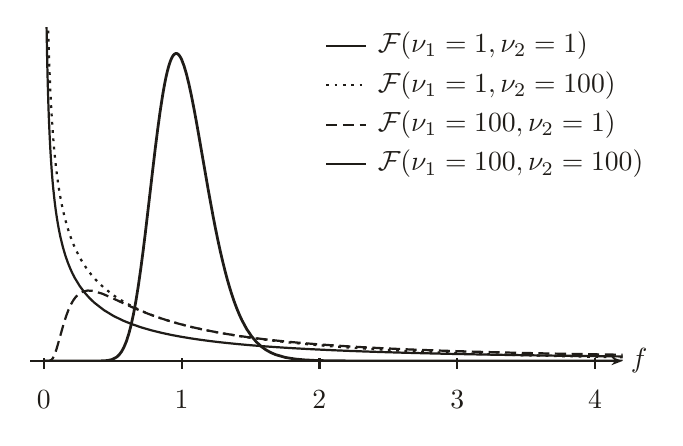
\begin{tikzpicture}[
  x=1.75cm,
  y=1.924cm,
  every node/.style={font=\normalsize, journalink},
  axis/.style={journalink, line width=0.8pt, -{Stealth[length=4pt]}},
  tick/.style={journalink, line width=0.8pt},
  curveaa/.style={journalink, line width=0.8pt},
  curveab/.style={journalink, line width=0.8pt,
                  dash pattern=on 1pt off 2pt},
  curveba/.style={journalink, line width=0.8pt,
                  dash pattern=on 4pt off 2pt},
  curvebb/.style={journalink, line width=1.0pt}
]
  %% ---- 四條密度曲線，超出縱向上界者由 clip 截斷 --------------------------
  \begin{scope}
    \clip (-0.1,0) rectangle (4.2,2.2);

    %% (nu1, nu2) = (1, 1)
    \draw[curveaa] plot coordinates {
      (0.0170,2.4000) (0.0181,2.3242) (0.0192,2.2548) (0.0203,2.1910) 
      (0.0214,2.1322) (0.0225,2.0776) (0.0235,2.0268) (0.0257,1.9350) 
      (0.0279,1.8539) (0.0301,1.7818) (0.0323,1.7169) (0.0344,1.6582) 
      (0.0366,1.6047) (0.0388,1.5558) (0.0432,1.4690) (0.0475,1.3941) 
      (0.0519,1.3288) (0.0562,1.2710) (0.0606,1.2194) (0.0649,1.1729) 
      (0.0693,1.1308) (0.0780,1.0572) (0.0867,0.9946) (0.0954,0.9406) 
      (0.1042,0.8933) (0.1129,0.8514) (0.1216,0.8139) (0.1390,0.7495) 
      (0.1564,0.6959) (0.1739,0.6503) (0.1913,0.6109) (0.2087,0.5764) 
      (0.2262,0.5459) (0.2610,0.4941) (0.2959,0.4516) (0.3307,0.4159) 
      (0.3656,0.3855) (0.4353,0.3361) (0.5050,0.2976) (0.5747,0.2666) 
      (0.6445,0.2411) (0.7142,0.2197) (0.7839,0.2015) (0.8536,0.1859) 
      (0.9233,0.1722) (0.9930,0.1603) (1.0628,0.1497) (1.1325,0.1403) 
      (1.2022,0.1318) (1.2719,0.1242) (1.3416,0.1174) (1.4113,0.1111) 
      (1.4811,0.1054) (1.5508,0.1002) (1.6205,0.0954) (1.6902,0.0910) 
      (1.7599,0.0869) (1.8296,0.0832) (1.8994,0.0797) (1.9691,0.0764) 
      (2.0388,0.0734) (2.1085,0.0705) (2.1782,0.0679) (2.2479,0.0654) 
      (2.3177,0.0630) (2.3874,0.0608) (2.4571,0.0587) (2.5268,0.0568) 
      (2.5965,0.0549) (2.6662,0.0532) (2.7360,0.0515) (2.8057,0.0499) 
      (2.8754,0.0484) (2.9451,0.0470) (3.0148,0.0457) (3.0845,0.0444) 
      (3.1543,0.0431) (3.2240,0.0420) (3.2937,0.0408) (3.3634,0.0398) 
      (3.4331,0.0388) (3.5028,0.0378) (3.5726,0.0368) (3.6423,0.0359) 
      (3.7120,0.0351) (3.7817,0.0342) (3.8514,0.0334) (3.9211,0.0327) 
      (3.9909,0.0319) (4.0606,0.0312) (4.1303,0.0305) (4.2000,0.0299)
    };

    %% (nu1, nu2) = (1, 100)
    \draw[curveab] plot coordinates {
      (0.0268,2.4000) (0.0289,2.3056) (0.0311,2.2211) (0.0333,2.1450) 
      (0.0355,2.0759) (0.0376,2.0129) (0.0398,1.9550) (0.0420,1.9016) 
      (0.0441,1.8522) (0.0485,1.7634) (0.0528,1.6856) (0.0572,1.6167) 
      (0.0615,1.5551) (0.0659,1.4996) (0.0702,1.4493) (0.0746,1.4034) 
      (0.0789,1.3612) (0.0876,1.2862) (0.0963,1.2214) (0.1050,1.1646) 
      (0.1137,1.1143) (0.1224,1.0693) (0.1311,1.0287) (0.1485,0.9582) 
      (0.1659,0.8987) (0.1833,0.8475) (0.2006,0.8029) (0.2180,0.7635) 
      (0.2354,0.7283) (0.2702,0.6680) (0.3050,0.6179) (0.3398,0.5752) 
      (0.3745,0.5384) (0.4093,0.5061) (0.4441,0.4774) (0.5136,0.4287) 
      (0.5832,0.3885) (0.6527,0.3546) (0.7223,0.3256) (0.7919,0.3003) 
      (0.8614,0.2780) (0.9310,0.2583) (1.0005,0.2406) (1.0701,0.2247) 
      (1.1396,0.2103) (1.2092,0.1972) (1.2787,0.1853) (1.3483,0.1743) 
      (1.4178,0.1641) (1.4874,0.1548) (1.5569,0.1462) (1.6265,0.1381) 
      (1.6961,0.1307) (1.7656,0.1237) (1.8352,0.1173) (1.9047,0.1112) 
      (1.9743,0.1055) (2.0438,0.1002) (2.1134,0.0952) (2.1829,0.0905) 
      (2.2525,0.0861) (2.3220,0.0819) (2.3916,0.0780) (2.4612,0.0743) 
      (2.5307,0.0708) (2.6003,0.0675) (2.6698,0.0644) (2.7394,0.0614) 
      (2.8089,0.0586) (2.8785,0.0560) (2.9480,0.0534) (3.0176,0.0510) 
      (3.0871,0.0488) (3.1567,0.0466) (3.2262,0.0446) (3.2958,0.0426) 
      (3.3654,0.0408) (3.4349,0.0390) (3.5045,0.0373) (3.5740,0.0357) 
      (3.6436,0.0342) (3.7131,0.0328) (3.7827,0.0314) (3.8522,0.0301) 
      (3.9218,0.0288) (3.9913,0.0276) (4.0609,0.0265) (4.1304,0.0254) 
      (4.2000,0.0243)
    };

    %% (nu1, nu2) = (100, 1)
    \draw[curveba] plot coordinates {
      (0.0040,0.0000) (0.0390,0.0005) (0.0565,0.0079) (0.0652,0.0177) 
      (0.0739,0.0327) (0.0827,0.0524) (0.0914,0.0761) (0.1089,0.1311) 
      (0.1439,0.2449) (0.1614,0.2947) (0.1788,0.3372) (0.1963,0.3722) 
      (0.2138,0.4002) (0.2313,0.4220) (0.2488,0.4383) (0.2663,0.4500) 
      (0.2837,0.4579) (0.3187,0.4647) (0.3537,0.4628) (0.4236,0.4443) 
      (0.4935,0.4168) (0.5635,0.3870) (0.6334,0.3579) (0.7033,0.3307) 
      (0.7733,0.3059) (0.8432,0.2834) (0.9131,0.2631) (0.9831,0.2449) 
      (1.0530,0.2285) (1.1229,0.2137) (1.1929,0.2004) (1.2628,0.1883) 
      (1.3327,0.1773) (1.4027,0.1673) (1.4726,0.1582) (1.5425,0.1499) 
      (1.6125,0.1422) (1.6824,0.1352) (1.7523,0.1287) (1.8223,0.1227) 
      (1.8922,0.1172) (1.9621,0.1120) (2.0321,0.1072) (2.1020,0.1028) 
      (2.1719,0.0986) (2.2419,0.0947) (2.3118,0.0910) (2.3817,0.0876) 
      (2.4517,0.0844) (2.5216,0.0814) (2.5915,0.0785) (2.6615,0.0758) 
      (2.7314,0.0733) (2.8013,0.0709) (2.8713,0.0686) (2.9412,0.0665) 
      (3.0111,0.0644) (3.0811,0.0625) (3.1510,0.0606) (3.2209,0.0589) 
      (3.2909,0.0572) (3.3608,0.0556) (3.4307,0.0541) (3.5007,0.0526) 
      (3.5706,0.0512) (3.6405,0.0499) (3.7105,0.0486) (3.7804,0.0474) 
      (3.8503,0.0462) (3.9203,0.0451) (3.9902,0.0440) (4.0601,0.0430) 
      (4.1301,0.0420) (4.2000,0.0410)
    };

    %% (nu1, nu2) = (100, 100)
    \draw[curvebb] plot coordinates {
      (0.0040,0.0000) (0.0739,0.0000) (0.1439,0.0000) (0.2138,0.0000) 
      (0.2837,0.0000) (0.3537,0.0000) (0.4236,0.0006) (0.4586,0.0026) 
      (0.4935,0.0090) (0.5285,0.0254) (0.5460,0.0401) (0.5635,0.0610) 
      (0.5810,0.0897) (0.5984,0.1277) (0.6159,0.1764) (0.6334,0.2370) 
      (0.6509,0.3103) (0.6684,0.3966) (0.6859,0.4956) (0.7033,0.6064) 
      (0.7208,0.7274) (0.7383,0.8565) (0.7733,1.1286) (0.7908,1.2654) 
      (0.8082,1.3985) (0.8257,1.5247) (0.8432,1.6411) (0.8607,1.7453) 
      (0.8694,1.7921) (0.8782,1.8351) (0.8869,1.8740) (0.8957,1.9088) 
      (0.9044,1.9393) (0.9131,1.9654) (0.9219,1.9871) (0.9306,2.0043) 
      (0.9394,2.0171) (0.9481,2.0255) (0.9568,2.0295) (0.9656,2.0293) 
      (0.9743,2.0250) (0.9831,2.0166) (0.9918,2.0045) (1.0006,1.9886) 
      (1.0180,1.9467) (1.0355,1.8925) (1.0530,1.8276) (1.0705,1.7540) 
      (1.0880,1.6734) (1.1055,1.5875) (1.1229,1.4980) (1.1929,1.1313) 
      (1.2278,0.9580) (1.2453,0.8765) (1.2628,0.7990) (1.2803,0.7260) 
      (1.2978,0.6574) (1.3153,0.5935) (1.3327,0.5342) (1.3502,0.4795) 
      (1.3677,0.4292) (1.3852,0.3832) (1.4027,0.3414) (1.4202,0.3033) 
      (1.4376,0.2690) (1.4726,0.2102) (1.5076,0.1630) (1.5425,0.1255) 
      (1.5775,0.0960) (1.6125,0.0731) (1.6474,0.0553) (1.6824,0.0417) 
      (1.7523,0.0234) (1.8223,0.0129) (1.8922,0.0071) (1.9621,0.0038) 
      (2.0321,0.0021) (2.1020,0.0011) (2.1719,0.0006) (2.2419,0.0003) 
      (2.3118,0.0002) (2.3817,0.0001) (2.4517,0.0000) (2.5216,0.0000) 
      (2.5915,0.0000) (2.6615,0.0000) (2.7314,0.0000) (2.8013,0.0000) 
      (2.8713,0.0000) (2.9412,0.0000) (3.0111,0.0000) (3.0811,0.0000) 
      (3.1510,0.0000) (3.2209,0.0000) (3.2909,0.0000) (3.3608,0.0000) 
      (3.4307,0.0000) (3.5007,0.0000) (3.5706,0.0000) (3.6405,0.0000) 
      (3.7105,0.0000) (3.7804,0.0000) (3.8503,0.0000) (3.9203,0.0000) 
      (3.9902,0.0000) (4.0601,0.0000) (4.1301,0.0000) (4.2000,0.0000)
    };
  \end{scope}

  %% ---- x 軸 --------------------------------------------------------------
  \draw[axis] (-0.1,0) -- (4.2,0);
  \node[anchor=west, inner sep=2.8pt] at (4.2,0) {$f$};

  \foreach \p in {0,1,2,3,4}
    \draw[tick] ([yshift=0.035cm]\p,0) -- ([yshift=-0.106cm]\p,0);
  \foreach \p in {0,1,2,3,4}
    \node[anchor=north] at ([yshift=-0.25cm]\p,0) {$\p$};

  %% ---- 圖例，右上角 ------------------------------------------------------
  %% 短線段由 x=2.05 到 x=2.336 (0.5cm)，文字起於 x=2.42。
  \draw[curveaa] (2.05,2.08) -- (2.336,2.08);
  \node[anchor=west, inner sep=0pt] at (2.42,2.08)
    {$\mathcal{F}(\nu_1=1,\nu_2=1)$};

  \draw[curveab] (2.05,1.82) -- (2.336,1.82);
  \node[anchor=west, inner sep=0pt] at (2.42,1.82)
    {$\mathcal{F}(\nu_1=1,\nu_2=100)$};

  \draw[curveba] (2.05,1.56) -- (2.336,1.56);
  \node[anchor=west, inner sep=0pt] at (2.42,1.56)
    {$\mathcal{F}(\nu_1=100,\nu_2=1)$};

  \draw[curvebb] (2.05,1.30) -- (2.336,1.30);
  \node[anchor=west, inner sep=0pt] at (2.42,1.30)
    {$\mathcal{F}(\nu_1=100,\nu_2=100)$};
\end{tikzpicture}
\end{document}
